\documentclass{article}

\usepackage{hyperref}
\usepackage[T1]{fontenc}
\usepackage{graphicx}
\usepackage{float}
\usepackage[utf8]{inputenc}


\title{%
Laboratorium 7\\
  \huge Kwadratury adaptacyjne}
\author{Mateusz Król}
\date{01/05/2024 r.}

\begin{document}
\maketitle

 
\section*{Zadanie 1.}
\textbf{Wiadomo, że $$ \int_{0}^{1} \frac{4}{1+x^2} \,dx = \pi.$$
\quad
Powyższą równość można wykorzystać do obliczenia przybliżonej
wartości $\pi$ poprzez całkowanie numeryczne. \\
\null\quad
Oblicz wartość powyższej całki, korzystając ze
złożonych kwadratur otwartej prostokątów (ang. mid-point rule), 
trapezów i Simpsona.}
\newpage
Wykres błędów względnych w zależności od liczby ewaluacji
funkcji podcałkowej dla kwadratury prostokątów, kwadratury trapezów,
kwadratury \textit{Simpson}'a:
\begin{figure}[H]
  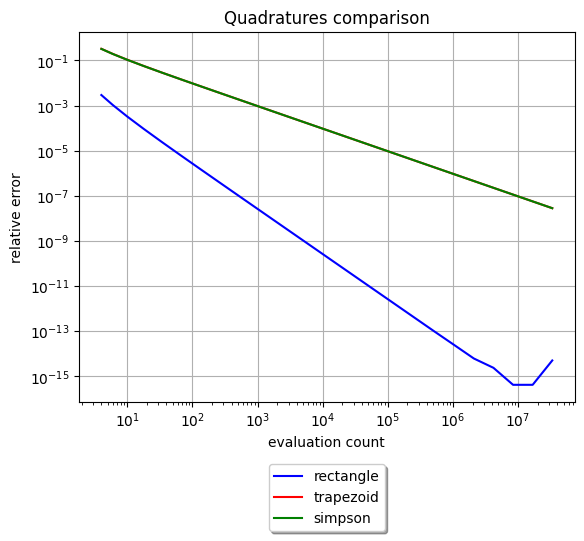
\includegraphics[width=\linewidth]{figures/quad.png}
\end{figure}
Wykres błędów względnych dla kwadratury trapezów i kwadratury \textit{Simpson}'a
pokrywa się.
\\\\
\null\quad
Z wykresu można odczytać, że zniżanie kroku poniżej $h \approx 10^{-7}$, 
nie zmniejsza już błędu kwadratury prostokątów. \\
Ten wynik zgadza się z wynikiem z \textit{Laboratorium 1}, w którym
wyznaczone $h_{min}$ wyniosło $10^{-6}$, $10^{-8}$.

\section*{Zadanie 2.}
\textbf{Oblicz wartość całki $$ \int_{0}^{1} \frac{4}{1+x^2} \,dx $$
metodą Gaussa-Legendre’a. Narysuj wykres wartości bezwzględnej
błędu względnego w zależności od liczby ewaluacji funkcji
podcałkowej, n + 1.}
\newpage
Wykres przedstawiający porównanie prawdziwych wartości funkcji 


\subsection*{Wnioski}
\null\quad 

\end{document}